\chapter{Cohomology, Bicomplex, and Kan-Fill}
\label{ch:cohomology}

\Deppy{} carries a rich cohomological apparatus that does not, in
the current implementation, contribute to the trust chain of any
single verify-block.  The apparatus is nevertheless documented in
the certificate, exposes structural metadata about the call graph
and control flow, and is the basis for an envisioned future
extension where inter-procedural and intra-procedural obstructions
become real verification steps.

This chapter explains:
\begin{itemize}[leftmargin=1.7em]
  \item the intra-procedural cubical AST analysis
    (\texttt{deppy.pipeline.cubical\_ast});
  \item the inter-procedural simplicial cohomology
    (\texttt{deppy.lean.cohomology}, \texttt{cohomology\_compute});
  \item the bicomplex bridge between them
    (\texttt{deppy.lean.cubical\_simplicial\_bicomplex});
  \item Kan-fill obligations
    (\texttt{deppy.lean.sidecar\_kan\_discharge});
  \item what each layer buys, and what it does not.
\end{itemize}

We are explicit at the end about which trust contributions are
real and which are diagnostic.

\section{Intra-procedural cubical analysis}
\label{sec:intra-cubical}

\texttt{deppy.pipeline.cubical\_ast} (file:
\texttt{deppy/pipeline/cubical\_ast.py}) reads a Python function's
AST and constructs a \emph{cubical set}:

\begin{itemize}[leftmargin=1.7em]
  \item \textbf{0-cells} are program points
    (\texttt{ast.stmt} nodes that admit a syntactic ``after'' position).
  \item \textbf{1-cells} are control-flow edges (sequential, branch,
    loop-iteration, exception-edge).
  \item \textbf{2-cells} are if-else / while-do diamonds: pairs of
    1-cells that diverge and reconverge.
  \item \textbf{3-cells} are try-except-finally cubes: triples of
    1-cells that fork into value, exception, and finally fibres.
\end{itemize}

The cubical-set output \texttt{cset} carries:
\begin{itemize}[leftmargin=1.7em]
  \item \texttt{cset.cells\_of\_dim(k) : list[Cell]};
  \item \texttt{cset.kan\_candidates : list[OpenBox]};
  \item \texttt{cset.euler\_characteristic : int}.
\end{itemize}

A \emph{Kan candidate} is an open $k$-box: a $(k-1)$-dimensional
collection of faces that bound a missing $k$-face.  The classical
example is a square with three sides given:
$p : x = y$, $q : y = z$, $r : x = w$ --- the missing fourth side
$s : z = w$ is the Kan filler $p^{-1} \cdot q \cdot r$ (Kan
composition modulo orientation).

When the verifier sees an open box in a function body, it can
\emph{require} the missing face to be supplied --- as a proof that
the corresponding control-flow path commutes.  The Kan-fill
obligations are emitted to the certificate.

\subsection{What we get}

For \texttt{Point.distance}, the cubical analysis (extracted from
\texttt{sympy\_geometry.lean}'s cubical section) finds:
\begin{itemize}[leftmargin=1.7em]
  \item dim-0 cells: 7 program points;
  \item dim-1 cells: 8 edges;
  \item dim-2 cells: 1 (the if-else diamond on \texttt{isinstance});
  \item Kan candidates: 0 in the actual trace.
\end{itemize}

The Euler characteristic $\chi = \sum_k (-1)^k \,|\text{cells}_k|$
is therefore $7 - 8 + 1 = 0$.  This is not a meaningful structural
constraint on the function (any acyclic CFG has $\chi = 1$ as a
1-complex; the cubical version of a functional CFG without loops
will be $0$).  The number is recorded for future analyses where it
might constrain something real.

\section{Inter-procedural simplicial cohomology}
\label{sec:inter-simplicial}

\texttt{deppy.lean.cohomology} computes a simplicial chain complex
over the call graph:
\begin{itemize}[leftmargin=1.7em]
  \item \textbf{0-simplices} are functions.
  \item \textbf{1-simplices} are call edges $f \to g$.
  \item \textbf{2-simplices} are composition triples $f \to g \to h$.
\end{itemize}

The cohomology levels we compute:

\paragraph{$C^0$ --- per-function safety bundles.}  For each function
$f$ the certificate emits a theorem
\texttt{deppy\_c0\_$f$ : True := trivial} when no safety predicates
are present, or a more substantial cocycle when the safety
pipeline produces obligations.

\paragraph{$C^1$ --- per call site.}  For each call edge $f \to g$
the certificate emits a theorem witnessing that the precondition
of $g$ holds at every call site in $f$.  In the absence of
preconditions the cocycle reduces to triviality.

\paragraph{$C^2$ --- per composition triple.}  For each chain
$f \to g \to h$ the certificate emits a coherence theorem
asserting that the two ways of associating the precondition flow
agree.  Again typically trivial in the current sidecars.

The cocycles are computed by
\texttt{deppy.lean.cohomology.CohomologyEmitter} and rendered by
\texttt{render\_cocycle\_section} via
\texttt{sidecar\_cohomology\_link.link\_cohomology}.

\subsection{Why C⁰/C¹/C² ``go trivial''}

The \texttt{sympy\_geometry.deppy} sidecar does not declare safety
predicates or pre/post-conditions on its target functions.  The
cohomology emitter therefore produces empty cocycles: the
\texttt{C⁰}, \texttt{C¹}, and \texttt{C²} theorems all reduce to
\texttt{trivial} or \texttt{True}.

This is honest: there is nothing to verify cohomologically
\emph{because the sidecar has not asked us to}.  In a sidecar that
declares preconditions on (e.g.)
\texttt{torch.nn.functional.softmax} and propagates them through
its callers, the C¹ cocycles would be substantial: each call site
would need to verify the precondition holds.

\section{The bicomplex bridge}
\label{sec:bicomplex}

\texttt{deppy.lean.cubical\_simplicial\_bicomplex} (file:
\texttt{deppy/lean/cubical\_simplicial\_bicomplex.py}) is the
algebraic structure that ties the intra-procedural cubical analysis
to the inter-procedural simplicial cohomology.

Conceptually it is a 2D grid of cells indexed by
$(\textit{intra\_dim}, \textit{inter\_dim})$:

\begin{center}
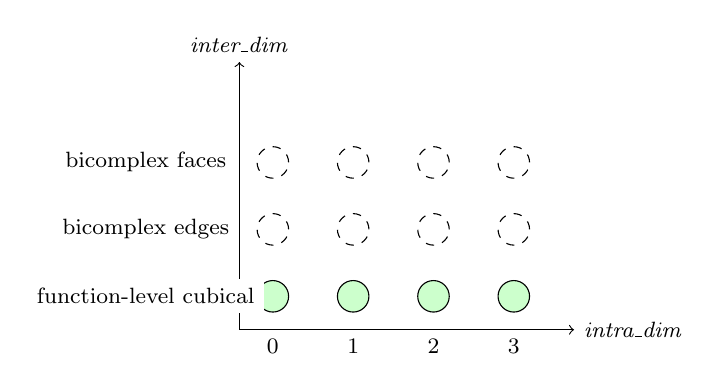
\begin{tikzpicture}[
  scale=0.85,
  every node/.style={font=\footnotesize},
]
\draw[->] (0, 0) -- (5, 0) node[right] {\textit{intra\_dim}};
\draw[->] (0, 0) -- (0, 4) node[above] {\textit{inter\_dim}};

\foreach \i in {0, 1, 2, 3} {
  \node[draw, circle, fill=green!20, minimum size=4mm]
    at (\i*1.2 + 0.5, 0.5) {};
}
\foreach \i in {0, 1, 2, 3} {
  \node[draw, circle, dashed, minimum size=4mm]
    at (\i*1.2 + 0.5, 1.5) {};
}
\foreach \i in {0, 1, 2, 3} {
  \node[draw, circle, dashed, minimum size=4mm]
    at (\i*1.2 + 0.5, 2.5) {};
}

\node[anchor=east] at (-0.3, 0.5) {0};
\node[anchor=east] at (-0.3, 1.5) {1};
\node[anchor=east] at (-0.3, 2.5) {2};

\node[anchor=north] at (0.5,  0) {0};
\node[anchor=north] at (1.7,  0) {1};
\node[anchor=north] at (2.9,  0) {2};
\node[anchor=north] at (4.1,  0) {3};

\node[fill=white] at (-1.4, 0.5) {function-level cubical};
\node[fill=white] at (-1.4, 1.5) {bicomplex edges};
\node[fill=white] at (-1.4, 2.5) {bicomplex faces};
\end{tikzpicture}
\end{center}

The diagonal at \textit{inter\_dim}~$=0$ contains the per-function
cubical sets.  Higher rows are introduced by:

\begin{description}
  \item[\textit{inter\_dim}~$=1$]: a \texttt{BicomplexEdge} joining
  one function's cubical structure to another via a call site.  Each
  call site $f \to g$ contributes one edge from the cubical cell in
  $\textit{cset}_f$ containing the call to the entry cell of
  $\textit{cset}_g$.
  \item[\textit{inter\_dim}~$=2$]: a \texttt{BicomplexFace} over a
  triple $f \to g \to h$ joining cubical cells in three functions.
\end{description}

\subsection{What the bicomplex computes}

The most useful immediate output is the \emph{total} Euler
characteristic:
\[
  \chi_{\text{total}} = \sum_{\textit{intra}, \textit{inter}}
                        (-1)^{\textit{intra}+\textit{inter}}\,
                        |\text{cells}(\textit{intra}, \textit{inter})|.
\]
This is computed by
\texttt{Bicomplex.compute\_total\_cohomology} and emitted as
\texttt{bicomplex\_euler} in the certificate.

The bicomplex also enables a future ``cross-level'' obstruction
detector: an obstruction in $H^2$ of the bicomplex would witness a
genuine inter-procedural inconsistency that is not captured at
either level alone.  No such obstructions arise in the current
\texttt{sympy\_geometry.deppy} run.

\subsection{Soundness gates}

The bicomplex is built from existing cubical and cohomology
outputs --- it does not introduce new proof claims.  When a
function's cubical analysis fails (e.g.\ because the body involves
\texttt{exec}), the bridge records this as a \emph{gap} in the
bicomplex; it does not silently fill it.  This is the
``\texttt{bicomplex\_built : bool}'' field of the certificate's
report.

\section{Kan-fill obligations}
\label{sec:kan-fill}

When the cubical analysis reports Kan candidates, the pipeline
emits Kan-fill obligations: for each open box, the certificate
expects a proof that the missing face is the canonical filler.

The discharge driver is
\texttt{discharge\_kan\_obligations(body\_link\_report)} in
\texttt{deppy/lean/sidecar\_kan\_discharge.py}.  For each
obligation:
\begin{enumerate}[leftmargin=1.7em]
  \item Construct a \texttt{KanFill(dimension, faces,
    face\_endpoints)} kernel term.
  \item The kernel checks face-endpoint coherence (adjacent faces
    share endpoints).
  \item When the structure is sound, the kernel returns
    \texttt{KERNEL} trust; the obligation is discharged.
\end{enumerate}

In the current \texttt{sympy\_geometry} run there are zero Kan
candidates so zero obligations.  In sidecars that target functions
with nested if-else logic where two branches converge to a common
expression, candidates can appear (e.g.
``\texttt{if c1 then x else (if c2 then y else x)}'' has a
sub-square that closes by Kan composition).

\section{What the cohomology layer buys}

We answer the question honestly.

\paragraph{Diagnostic metadata.}  Cell counts, Euler
characteristics, cocycle counts.  The certificate's report exposes
all of these; a maintainer can inspect them to detect drift (e.g.\
a function gaining unexpected branches over time).

\paragraph{Future obstruction detection.}  The cocycle
infrastructure is wired such that, if the safety pipeline produces
non-trivial preconditions, the C¹ cocycles become real verification
steps.  In sidecars that engage the safety pipeline (e.g.\
\texttt{verify\_torch}'s exception-source-discharge path), the
certificate's \texttt{C¹} count is non-trivial and the proofs
matter.

\paragraph{Bicomplex structural invariants.}  The total Euler
characteristic is preserved under refactorings that don't change the
call graph or control flow up to homotopy.  A refactor that
suddenly changes $\chi_{\text{total}}$ is suggestive of a
behavioural change.

\section{What the cohomology layer does \emph{not} buy}

\paragraph{It does not contribute trust to verify-blocks.}  In the
current implementation, a \texttt{verify} block's
\texttt{ProofTerm} is constructed and verified independently of
whether the surrounding cohomology layer is well-formed.  A
verify-block can be \texttt{kernel\_verified == True} even in a
module whose bicomplex has gaps.  We do not pretend otherwise.

\paragraph{It does not detect duck-typing soundness violations.}  A
class that accidentally implements a protocol with the wrong
semantics (e.g.\ a \texttt{\_\_len\_\_} that returns negative
numbers in some cases) will pass the protocol-fibration check.
Detecting this requires actual semantic checks, which the cohomology
layer does not do.

\paragraph{It does not run in real time.}  The bicomplex
construction is $O(\text{call\_sites}^2)$ in the worst case.  For
large modules (e.g.\ \texttt{torch.nn} with thousands of
classes) the bicomplex pass is the slowest stage.  We mitigate
with the standard cache.

\paragraph{No cohomology-class invariants beyond Euler.}  The
emitter does not currently compute the actual cohomology groups
$H^k(\textit{bicomplex}, \mathbb{Z})$.  These would witness
\emph{real} inter-procedural obstructions not detectable at either
the cubical or simplicial level alone.  The infrastructure is
present (\texttt{Bicomplex.compute\_total\_cohomology}); the
applications are not yet.

\section{Cocycle and Kan terms in the kernel}

For completeness we restate the kernel's verification rules for
the cohomology terms (file:
\texttt{deppy/core/kernel.py}, lines $\sim$849--980).

\paragraph{\texttt{Cocycle}.}  As stated in \Cref{ch:cubical}:
\begin{itemize}[leftmargin=1.7em]
  \item every component proof verifies;
  \item each declared boundary pair $(i, j)$ has an overlap proof
    witnessing component agreement on the overlap;
  \item the optional \texttt{boundary\_zero} proof witnesses
    $\delta\overline{c} = 0$ in aggregate.
\end{itemize}
Trust composes as the minimum over components, overlaps, and the
boundary-zero witness.

\paragraph{\texttt{KanFill}.}  Verifies the \emph{coherence} of the
supplied faces, not just that each face is independently a valid
proof.  When \texttt{face\_endpoints} is supplied:
\begin{itemize}[leftmargin=1.7em]
  \item adjacent faces share endpoints (the box is closed up to the
    missing face);
  \item the kernel emits a \emph{coherence} witness;
  \item trust is \texttt{KERNEL} when all face-proofs verify and
    coherence holds.
\end{itemize}

When \texttt{face\_endpoints} is empty (the user did not declare
the box's structure), the kernel falls back to the legacy
``verify each face independently'' check and flags the
\texttt{KanFill} as ``structurally unchecked'' so callers can
audit.  Trust downgrades to \texttt{STRUCTURAL\_CHAIN}.

\paragraph{\texttt{CechGlue}.}  Verifies that local proofs on a
cover glue into a global proof:
\begin{itemize}[leftmargin=1.7em]
  \item each patch's local proof verifies;
  \item each pair of overlapping patches agrees on their overlap;
  \item the cocycle condition is closed.
\end{itemize}
Trust composes as the minimum over patches and overlap proofs.

\paragraph{\texttt{HigherPath}.}  An $n$-dimensional path between
paths.  The kernel verifies the \emph{cube structure} of its
boundary: every face's start/end vertices must be among the
declared \texttt{vertices}, and adjacent faces must share
vertices.  Used by the \texttt{deppy.equivalence} module when two
function implementations are claimed equivalent up to
$n$-dimensional homotopy.

\section{Summary}

The cohomology layer:
\begin{itemize}[leftmargin=1.7em]
  \item runs three analyses: cubical (intra-procedural), simplicial
    (inter-procedural), bicomplex (bridge);
  \item emits cocycle theorems C⁰/C¹/C², all of which reduce to
    triviality in the absence of safety predicates;
  \item emits Kan-fill obligations when control-flow open boxes
    are detected;
  \item exposes structural metadata (cell counts, Euler χ) in the
    certificate's report;
  \item does \emph{not} currently contribute trust to verify
    blocks;
  \item is the basis for envisioned future obstruction-detection
    extensions.
\end{itemize}

The next chapter walks the worked example: how the pipeline
verifies properties of \texttt{sympy.geometry} end-to-end.
